% =====================================================================
%  Shared sections (model, stability, control, swing-up) used by build_full_report.py and build_phase_reports.py
%  (layout follows the senior reference report: title page, contents,
%   numbered sections, code listings, tabulation, conclusion, contributions)
% =====================================================================
\documentclass[12pt,a4paper]{article}
\usepackage[a4paper,margin=1in]{geometry}
\usepackage[T1]{fontenc}
\usepackage{lmodern}
\usepackage{amsmath,amssymb,bm}
\usepackage{graphicx,float,booktabs,array,multirow}
\usepackage{xcolor}
\usepackage{algorithm}
\usepackage{algpseudocode}
\usepackage{fancyhdr}
\usepackage{enumitem}
\usepackage{caption}
\usepackage[hidelinks]{hyperref}

\pagestyle{fancy}
\fancyhf{}
\renewcommand{\headrulewidth}{0.6pt}
\fancyfoot[C]{\thepage}
\setlength{\headheight}{14.5pt}
\setlength{\parskip}{4pt}
\setlength{\parindent}{0pt}
\newcommand{\Nm}{\,\mathrm{N\,m}}
\captionsetup{font=small}

\begin{document}

\begin{titlepage}
\centering
\vspace*{2cm}

\includegraphics[width=4.2cm]{figures/logo-000.jpg}\\[3cm]
{\Huge Systems Thinking Project}\\[0.5cm]
{\Large Acrobot}\\[0.25cm]
{\large Phase 3: Control Around the Equilibria}\\[2.2cm]
\begin{tabular}{cc}
\textbf{Author:} Bhargav & \textbf{Author:} Sreekar\\
ID: 2025102061 & ID: 2025102074\\[0.8cm]
\textbf{Author:} Kaushik & \textbf{Author:} Divijat\\
ID: 2025102071 & ID: 2025102040
\end{tabular}
\vfill
{\large November 11, 2026}
\end{titlepage}

\tableofcontents
\newpage

\section{Introduction}
% =====================================================================
\subsection{What is an Acrobot?}
An acrobot is a two-link pendulum that hangs from a fixed pivot. The first link (the ``shoulder'' link) is free to rotate about the pivot; the second link is joined to the end of the first at the ``elbow''. The only motor sits at the elbow, so the shoulder is \emph{passive}. It is the robot version of a gymnast on a high bar who can only swing the legs at the hips. Because there are two degrees of freedom but only one actuator, the acrobot is a standard example of an \emph{underactuated} system [1], [2].

\subsection{Model}
The configuration is described by two generalised coordinates: $q_1$, the angle of link~1 from the downward vertical, and $q_2$, the angle of link~2 relative to link~1. The full state contains the angles and their rates:
\[
\mathbf q=\begin{bmatrix}q_1\\q_2\end{bmatrix},\qquad
\mathbf x=\begin{bmatrix}q_1\\q_2\\\dot q_1\\\dot q_2\end{bmatrix}.
\]
\begin{figure}[H]
\centering
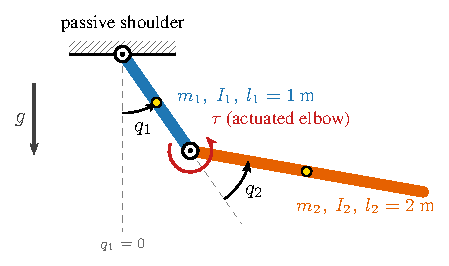
\includegraphics[width=0.42\textwidth]{figures/acrobot_diagram.pdf}
\caption{The acrobot: passive shoulder at the pivot, motor torque $\tau$ at the elbow; dots mark the centres of mass.}
\label{fig:acrobot}
\end{figure}

\subsection{Equations of Motion}
The dynamics (given in the Phase~1 helper and verified in Phase~1) are
\begin{equation}
M(q)\,\ddot q+C(q,\dot q)\,\dot q=\tau_g(q)+B\,\tau,\qquad B=\begin{bmatrix}0\\1\end{bmatrix},\qquad |\tau|\le 20\Nm .\label{eq:eom}
\end{equation}

\textbf{$\tau$ (Input Torque):} the torque of the elbow motor, the only quantity we command. $B=[0,\,1]^T$ says it acts on the elbow equation only.

\textbf{$M(q)$ (Inertia Matrix):} the resistance to angular acceleration. It depends on the elbow angle because the mass distribution changes as the arm folds:
\begin{equation}
M(q)=\begin{bmatrix}2.663+2\cos q_2 & 1.33+\cos q_2\\ 1.33+\cos q_2 & 1.33\end{bmatrix},\qquad \det M=1.7729-\cos^2q_2\ge0.7729>0 .
\end{equation}

\textbf{$C(q,\dot q)$ (Coriolis Matrix):} the coupling forces between the links (centrifugal and Coriolis effects):
\begin{equation}
C(q,\dot q)=\sin q_2\begin{bmatrix}-2\dot q_2 & -\dot q_2\\ \dot q_1 & 0\end{bmatrix}.
\end{equation}

\textbf{$\tau_g(q)$ (Gravity Torque):} the torque that gravity exerts on each joint, $\tau_g=-\partial U/\partial q$, with potential energy $U$:
\begin{equation}
U=-14.715\cos q_1-9.81\cos(q_1+q_2),\qquad
\tau_g(q)=-9.81\begin{bmatrix}1.5\sin q_1+\sin(q_1+q_2)\\ \sin(q_1+q_2)\end{bmatrix}.
\end{equation}

\textbf{System Parameters:}
\begin{gather*}
m_1=m_2=1\,\mathrm{kg},\qquad l_1=1\,\mathrm m,\qquad l_2=2\,\mathrm m,\qquad l_{c1}=0.5\,\mathrm m,\qquad l_{c2}=1\,\mathrm m,\\
I_1=0.083\,\mathrm{kg\,m^2},\qquad I_2=0.33\,\mathrm{kg\,m^2},\qquad g=9.81\,\mathrm{m\,s^{-2}}.
\end{gather*}

\subsection{Equilibria and Linear Model (from Phase 1)}
With $\tau^*=0$ the equilibria satisfy $\tau_g(q^*)=0$, i.e.\ $\sin q_1^*=0$ and $\sin(q_1^*+q_2^*)=0$. This gives four postures:
\begin{table}[H]
\centering
\caption{The four equilibria}
\begin{tabular}{|c|c|c|c|l|}
\hline
 & Posture & $(q_1^*,q_2^*)$ & $U$ [J] & Description\\ \hline
$E_1$ & down--down & $(0,0)$ & $-24.525$ & both links hanging\\
$E_2$ & down--up & $(0,\pi)$ & $-4.905$ & link 1 down, link 2 up\\
$E_3$ & up--up & $(\pi,0)$ & $+24.525$ & fully upright (target)\\
$E_4$ & up--down & $(\pi,\pi)$ & $+4.905$ & link 1 up, link 2 down\\ \hline
\end{tabular}
\end{table}
Linearizing about each equilibrium with $\tilde x=x-x^*$ gives
\begin{equation}
\dot{\tilde x}=A\tilde x+B_\ell\tilde\tau,\qquad A=\begin{bmatrix}0&I\\P&0\end{bmatrix},\qquad B_\ell=\begin{bmatrix}0\\r\end{bmatrix},\label{eq:lin}
\end{equation}
with $P=M(q^*)^{-1}K(q^*)$ and $r=M(q^*)^{-1}B$,
where $K=\partial\tau_g/\partial q$. The transfer functions from $\tau$ to the angles are
\begin{gather}
G_1(s)=\frac{r_1s^2+(P_{12}r_2-P_{22}r_1)}{\Delta(s)},\qquad
G_2(s)=\frac{r_2s^2+(P_{21}r_1-P_{11}r_2)}{\Delta(s)},\label{eq:tf}\\
\Delta(s)=s^4-\operatorname{tr}(P)\,s^2+\det P .\nonumber
\end{gather}
\begin{table}[H]
\centering
\caption{Transfer functions at the four equilibria (Phase 1)}
\label{tab:tf}
\small
\begin{tabular}{|c|l|l|l|}
\hline
 & $\Delta(s)$ & $N_1(s)$ ($\tau\to q_1$) & $N_2(s)$ ($\tau\to q_2$)\\ \hline
$E_1$ & $s^4+42.2410\,s^2+186.7719$ & $-3.0147\,(s^2+4.2103)$ & $6.0332\,(s^2+5.2595)$\\
$E_2$ & $s^4+8.4025\,s^2-186.7719$ & $-0.4270\,(s^2-29.7273)$ & $0.8578\,(s^2+7.3982)$\\
$E_3$ & $s^4-42.2410\,s^2+186.7719$ & $-3.0147\,(s^2-4.2103)$ & $6.0332\,(s^2-5.2595)$\\
$E_4$ & $s^4-8.4025\,s^2-186.7719$ & $-0.4270\,(s^2+29.7273)$ & $0.8578\,(s^2-7.3982)$\\ \hline
\end{tabular}
\end{table}

\subsection{Objective}
Design controllers that stabilize the acrobot at the upright equilibrium $E_3$ and at least one other equilibrium, and justify the design choices. Characterize the limits of each controller: how far from the equilibrium it still works with $\tau_{\max}=20\Nm$.

Phase~2 showed that $E_1$ is only marginally stable, that $E_2$, $E_3$, $E_4$ are unstable (1, 2 and 1 RHP poles), and that one measured angle cannot stabilize $E_3$ with PD feedback. That result guides the design here.

% =====================================================================
\section{Control Around the Equilibria}
% =====================================================================
\subsection{Controller Design}
The rank of $\mathcal C$ is 4 at every equilibrium, so all four states can be fed back. Including the torque limit, every controller has the form
\begin{equation}
\tau=\operatorname{sat}(-K\tilde x),\qquad \tilde x=[\tilde q_1,\ \tilde q_2,\ \dot q_1,\ \dot q_2]^T,\qquad |\tau|\le20\Nm .
\end{equation}
The controllers used are:
\begin{itemize}
\item \textbf{LQR} at the upright $E_3$, at $E_2$ and at $E_4$;
\item \textbf{pole placement} at $E_3$, for comparison;
\item \textbf{PD on the elbow angle only} at $E_1$.
\end{itemize}

\subsection{Linear Quadratic Regulator (LQR)}
$K$ minimizes a cost that penalizes both the state error and the torque:
\begin{equation}
J=\int_0^\infty\big(\tilde x^TQ\tilde x+R\,\tau^2\big)\,dt,\qquad A^TS+SA-SB_\ell R^{-1}B_\ell^TS+Q=0,\qquad K=R^{-1}B_\ell^TS .
\end{equation}
\textbf{Expected performance of LQR:}
\begin{itemize}
\item \textbf{Stability:} guaranteed for any $Q\succeq0$, $R>0$ when $(A,B_\ell)$ is controllable.
\item \textbf{Robustness:} phase margin $\ge60^\circ$ and gain margin $[\frac12,\infty)$ [7].
\item \textbf{Tuning:} $Q=I$ weighs 1~rad of angle like 1~rad/s of rate. A smaller $R$ makes the controller faster but demands more torque, so $R$ trades speed against saturation.
\end{itemize}

\subsubsection{Choice of $R$}
For each $R$ we simulated the nonlinear saturated loop from a grid of initial offsets and counted how many were recovered (Fig.~\ref{fig:design}).
\begin{itemize}
\item \textbf{$E_3$:} the recovered area stays at 16--20\% of a $\pm60^\circ$ grid for $10^{-3}\le R\le1$, while the fastest pole moves from $-10$ to $-214$~s$^{-1}$. The limit is $\tau_{\max}$, not the tuning. $R=0.03$ is the knee: 93\% of the best area with a fastest pole of $-40$.
\item \textbf{$E_2$:} the region collapses for $R>0.3$ ($99\%\to90\%\to20\%$), so $R=0.1$.
\item \textbf{$E_4$:} the area peaks at $R\approx0.1$--$0.18$, so $R=0.1$.
\end{itemize}
\begin{figure}[H]
\centering
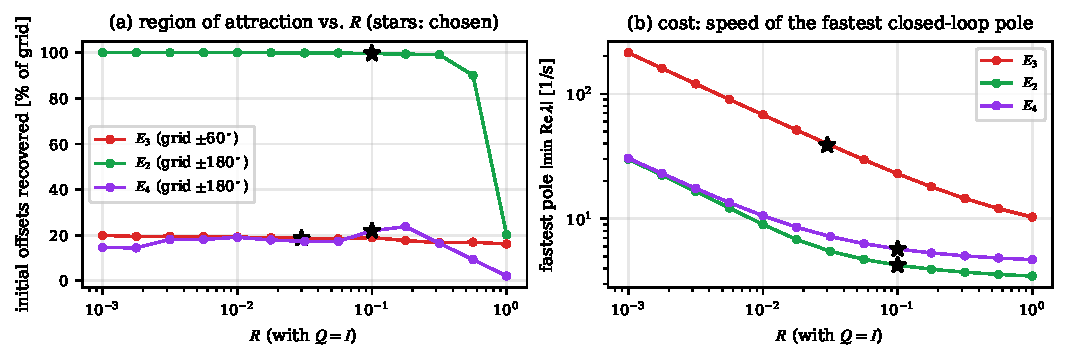
\includegraphics[width=\textwidth]{figures/fig_design.pdf}
\caption{Weight selection ($Q=I$): (a) share of offsets recovered; (b) fastest closed-loop pole. Stars: chosen $R$.}
\label{fig:design}
\end{figure}

\subsection{Pole Placement at $E_3$ (Comparison)}
Placing the poles at $\{-3,-4,-5,-6\}$ gives $K=[-322.9,\,-134.6,\,-138.1,\,-66.0]$. It settles faster from $2^\circ$ ($1.3$~s vs $4.1$~s) and with less torque ($11.3$ vs $17.6\Nm$), but recovers a smaller region ($20\%$ vs $26\%$ of $\pm40^\circ$; $5^\circ$ vs $6^\circ$ along $q_1$). LQR is therefore kept for $E_3$.

\subsection{$E_1$: PD on the Elbow Angle Only}
At $E_1$ the zeros of $G_2$ are imaginary ($\pm j2.29$), so the PD sign conflict found at $E_3$ in Phase~2 does not arise and one angle suffices:
\begin{equation}
\tau=-K_p\tilde q_2-K_d\dot q_2,\qquad K_p=-5,\quad K_d=0.4,
\end{equation}
the pair with the best decay rate on a $(K_p,K_d)$ grid ($\max\operatorname{Re}\lambda=-0.52$).
\textbf{Proof of stability (energy shaping, LaSalle [4]):}
\begin{gather}
V_c=E-E^*+\tfrac12K_p\tilde q_2^{\,2},\qquad \dot V_c=-K_d\,\dot q_2^{\,2}\le0,\\
\nabla^2\big(U+\tfrac12K_p\tilde q_2^{\,2}\big)\big|_{E_1}\ \text{has eigenvalues}\ 0.760,\ 28.575>0 .\nonumber
\end{gather}
$V_c$ has a strict minimum at $E_1$ and never increases, and $\dot q_2\equiv0$ only at $E_1$, so $E_1$ is asymptotically stable. Pure damping ($K_p=0$) decays $19\times$ more slowly.

\subsection{Designed Controllers}
\begin{table}[H]
\centering
\caption{Phase 3 controllers and their closed-loop poles}
\label{tab:ctrl}
\small
\resizebox{\textwidth}{!}{\begin{tabular}{|l|l|l|l|}
\hline
Controller & Design & $K=[k_{q_1},k_{q_2},k_{\dot q_1},k_{\dot q_2}]$ & Closed-loop poles\\ \hline
$E_3$ LQR & $Q=I$, $R=0.03$ & $[-503.0,\,-203.9,\,-218.3,\,-101.5]$ & $-39.86,\,-2.25\pm0.10j,\,-1.34$\\
$E_3$ pole placement & $\{-3,-4,-5,-6\}$ & $[-322.9,\,-134.6,\,-138.1,\,-66.0]$ & $-6,\,-5,\,-4,\,-3$\\
$E_2$ LQR & $Q=I$, $R=0.1$ & $[6.60,\,46.49,\,5.23,\,13.24]$ & $-4.26,\,-2.40,\,-1.24\pm4.16j$\\
$E_4$ LQR & $Q=I$, $R=0.1$ & $[-49.31,\,38.91,\,-13.19,\,6.10]$ & $-5.73,\,-3.21,\,-0.96\pm3.08j$\\
$E_1$ elbow PD & $K_p=-5$, $K_d=0.4$ & $[0,\,-5,\,0,\,0.4]$ & $-0.69\pm2.31j,\,-0.52\pm2.14j$\\ \hline
\end{tabular}}
\end{table}

\subsection{Limits with $\tau_{\max}=20\Nm$}
\subsubsection{Guaranteed Region}
Inside $\Omega_c=\{\tilde x^TS\tilde x\le c\}$ the command never saturates if
\begin{equation}
c^*=\frac{\tau_{\max}^2}{KS^{-1}K^T},\qquad \dot V=-\tilde x^T(Q+K^TRK)\tilde x<0\ \text{ on }\Omega_{c^*}.
\end{equation}
At rest this guarantees $0.72^\circ/1.66^\circ$ ($E_3$), $45.6^\circ/19.9^\circ$ ($E_2$) and $20.0^\circ/23.1^\circ$ ($E_4$) along $q_1$/$q_2$. The bound is conservative because short saturation is usually survived.

\subsubsection{Simulated Region of Attraction}
The real limits come from simulating the nonlinear saturated loop from a grid of initial offsets at rest. A start counts as recovered if it ends within $1^\circ$ and $0.05$~rad/s of $q^*$. The fast integrator used for the grids matches PyBullet on 100\% of random points and 96\% of boundary points.
\begin{figure}[H]
\centering
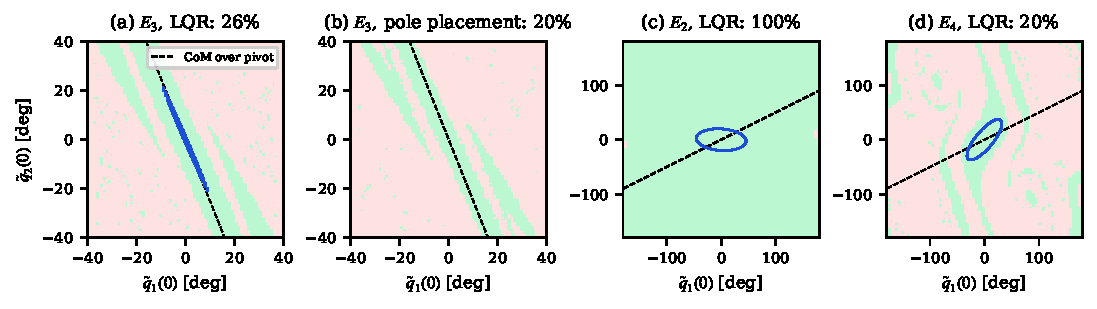
\includegraphics[width=\textwidth]{figures/fig_roa.pdf}
\caption{Region of attraction (green: recovered). Blue ellipse: guaranteed region. Dashed: offsets with the centre of mass over the pivot.}
\label{fig:roa}
\end{figure}
\begin{table}[H]
\centering
\caption{How far from the equilibrium each controller still works}
\label{tab:limits}
\small
\resizebox{\textwidth}{!}{\begin{tabular}{|l|c|c|c|c|c|}
\hline
Controller & Recovered (grid) & $|\tilde q_1(0)|$ alone & $|\tilde q_2(0)|$ alone & Shoulder kick & Settling\\ \hline
$E_3$ LQR & 26\% ($\pm40^\circ$) & $6^\circ$ & $13^\circ$ & $0.20$ rad/s & $4.1$ s\\
$E_3$ pole placement & 20\% ($\pm40^\circ$) & $5^\circ$ & $9^\circ$ & $0.15$ rad/s & $1.3$ s\\
$E_2$ LQR & 99.7\% ($\pm180^\circ$) & $175^\circ$ & $180^\circ$ & $\ge8$ rad/s & $3.0$ s\\
$E_4$ LQR & 20.5\% ($\pm180^\circ$) & $35^\circ$ & $55^\circ$ & $2.1$ rad/s & $3.6$ s\\
$E_1$ elbow PD & 77.8\% ($\pm180^\circ$) & $40^\circ$ & $115^\circ$ & $2.15$ rad/s & $12.8$ s\\ \hline
\end{tabular}}
\end{table}

\textbf{Why the upright region is a thin band.} Linearizing $\tau_g$ at $E_3$:
\begin{equation}
\tau_{g,1}=9.81\,(2.5\,\tilde q_1+\tilde q_2).
\end{equation}
Gravity pushes the passive shoulder in proportion to the horizontal offset of the total centre of mass. The motor can only counter this through the elbow coupling. Along $\tilde q_2=-2.5\,\tilde q_1$ there is no shoulder torque, and the region reaches the grid edge ($\ge43^\circ$). Across that line, $20\Nm$ is used up after about $6^\circ$.

\subsection{Time Responses}
\begin{figure}[H]
\centering
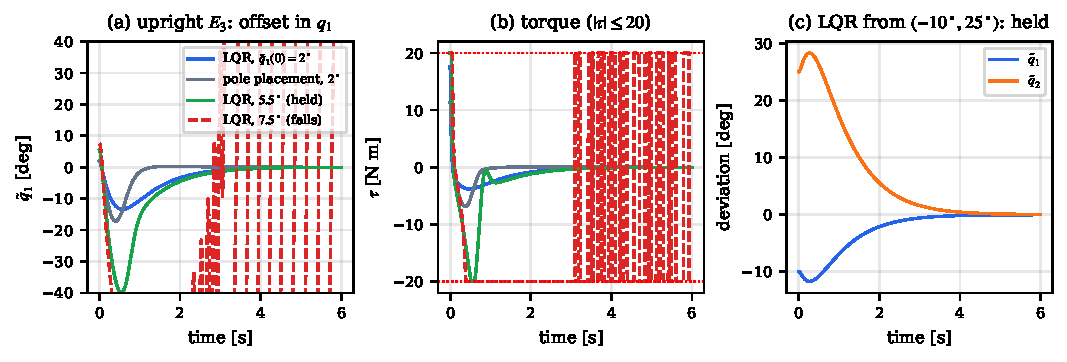
\includegraphics[width=\textwidth]{figures/fig_e3.pdf}
\caption{$E_3$ in PyBullet: LQR is held from $5.5^\circ$ and falls from $7.5^\circ$; a CoM-balanced offset $(-10^\circ,25^\circ)$ is held with only $3.3\Nm$.}
\label{fig:e3}
\end{figure}
\begin{figure}[H]
\centering
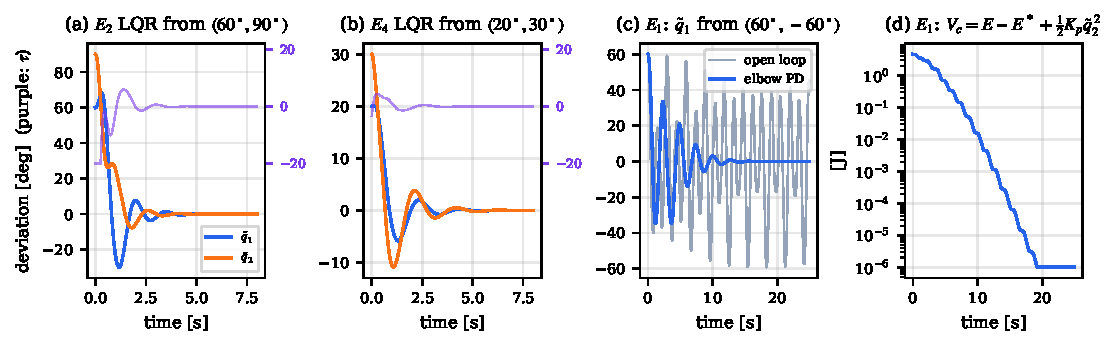
\includegraphics[width=\textwidth]{figures/fig_others.pdf}
\caption{(a) $E_2$ and (b) $E_4$ with LQR; (c) $E_1$ with elbow PD vs.\ open loop; (d) $V_c$ decreasing along the $E_1$ run.}
\label{fig:others}
\end{figure}
\textbf{Observations:}
\begin{itemize}
\item \textbf{Settling time:} pole placement settles fastest at $E_3$, but LQR rescues a larger region. $E_1$ is slowest ($12.8$~s) because its slow mode barely moves the elbow.
\item \textbf{Control effort:} at $E_3$ even a $2^\circ$ offset needs $17.6\Nm$, close to the limit, which explains the small region. At $E_4$ the peak is only $4.5\Nm$.
\item \textbf{Steady-state error:} zero for every controller (each converges to $q^*$ within $0.001^\circ$).
\end{itemize}

% =====================================================================
% =====================================================================
\section{Simulations and Code}
% =====================================================================
\subsection{PyBullet Simulator}
All simulations use the full nonlinear model in PyBullet with an interactive dashboard (Fig.~\ref{fig:dash}). The user picks an equilibrium, an initial condition (slider, typed value or by dragging the arm) and a controller: open loop, full-state LQR, pole placement, elbow PD (for $E_1$), or the Phase 2 single-angle controllers. The dashboard shows $\tilde q(t)$, $\tau(t)$ and the closed-loop poles live. File: \texttt{phase3/acrobot\_phase3\_sim.py}; instructions in \texttt{phase3/README.md}.
\begin{figure}[H]
\centering
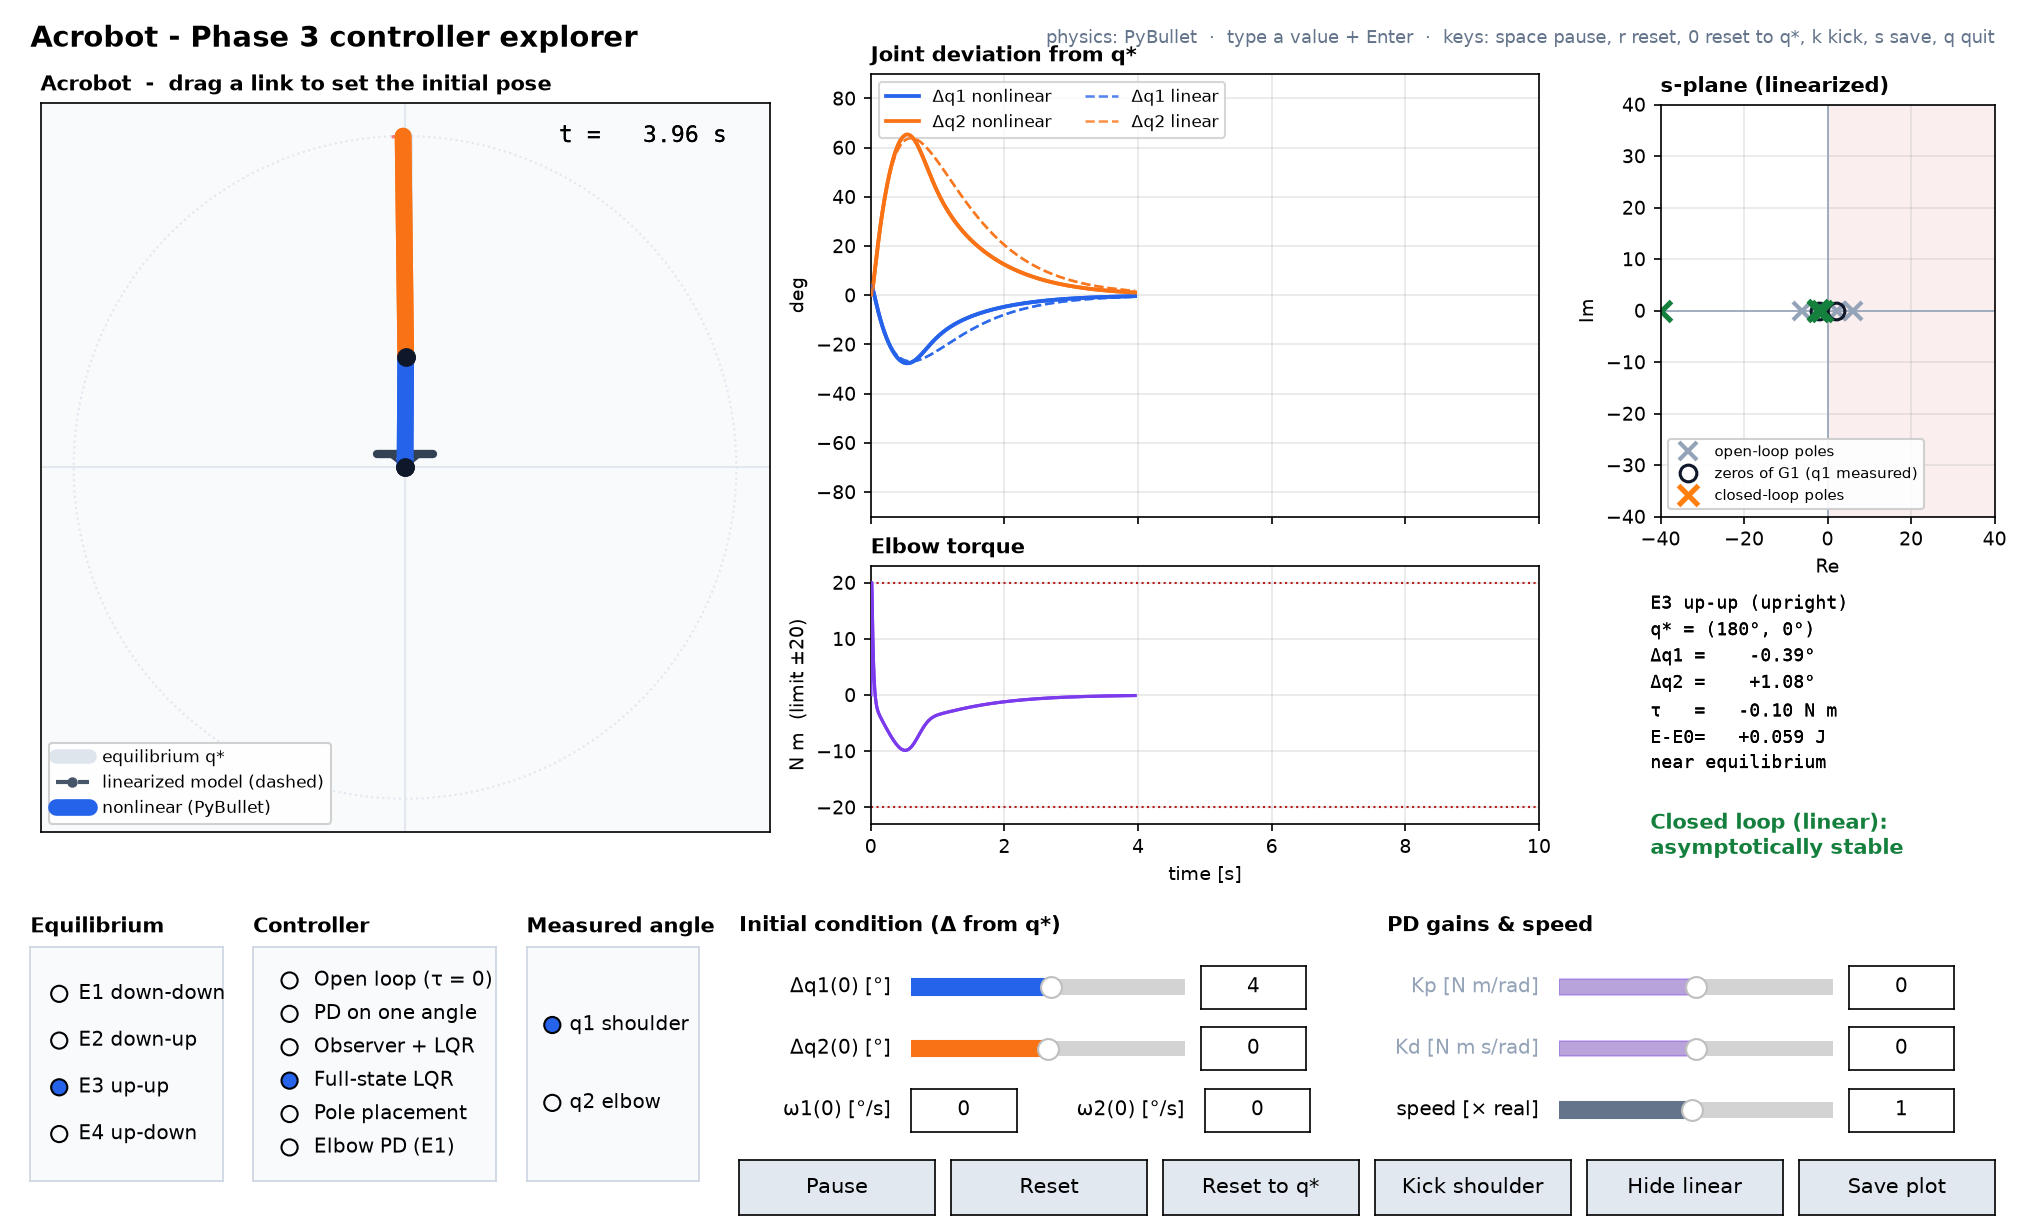
\includegraphics[width=\textwidth]{figures/dashboard_p3.png}
\caption{Phase 3 dashboard: full-state LQR catching the upright from $4^\circ$.}
\label{fig:dash}
\end{figure}

\subsection{MATLAB Codes}
It designs every controller (\texttt{lqr}, \texttt{place}), prints the gains, poles and guaranteed regions, runs the nonlinear saturated loops with \texttt{ode45}, and maps the regions of attraction. Gains, poles and guaranteed regions match the tables above exactly.

The files are listed below; the algorithms they implement follow as pseudo-code.
\begin{table}[H]
\centering
\caption{MATLAB files}
\resizebox{\textwidth}{!}{\begin{tabular}{|l|l|}
\hline
File & Purpose\\ \hline
\texttt{Acrobot\_Nonlinear\_Dynamics.m} & nonlinear model $\dot x=f(x,\tau)$ with the $20\Nm$ limit (Phase 1)\\
\texttt{Acrobot\_Linearize.m} & $A$, $B_\ell$ at an equilibrium (Phase 1)\\
\texttt{Acrobot\_Phase3\_Design.m} & the controllers (LQR, pole placement, elbow PD)\\
\texttt{Acrobot\_Phase3\_Main.m} & guaranteed regions, nonlinear runs, region-of-attraction maps\\ \hline
\end{tabular}}
\end{table}

\begin{algorithm}[H]
\caption{Nonlinear dynamics $\dot x=f(x,\tau)$ (\texttt{Acrobot\_Nonlinear\_Dynamics.m}) and linearization (\texttt{Acrobot\_Linearize.m})}
\label{alg:model}
\begin{algorithmic}[1]
\Function{Dynamics}{$x=[q_1,q_2,\dot q_1,\dot q_2]$, $\tau$}
  \State $\tau\gets\max(-20,\min(20,\tau))$ \Comment{motor limit}
  \State build $M(q)$, $C(q,\dot q)$ and $\tau_g(q)$ from the given model
  \State solve $M\,\ddot q=\tau_g+B\tau-C\dot q$ for $\ddot q$ \Comment{backslash, never $M^{-1}$}
  \State \Return $[\dot q;\ \ddot q]$
\EndFunction
\Function{Linearize}{$q^*$}
  \State $K\gets\partial\tau_g/\partial q$ at $q^*$; \quad $P\gets M(q^*)^{-1}K$; \quad $r\gets M(q^*)^{-1}B$
  \State \Return $A=\begin{bmatrix}0&I\\P&0\end{bmatrix}$, $B_\ell=\begin{bmatrix}0\\r\end{bmatrix}$
\EndFunction
\end{algorithmic}
\end{algorithm}

\begin{algorithm}[H]
\caption{Controller design and limits (\texttt{Acrobot\_Phase3\_Design.m}, \texttt{Acrobot\_Phase3\_Main.m})}
\label{alg:p3}
\begin{algorithmic}[1]
\For{each design (LQR at $E_2,E_3,E_4$; pole placement at $E_3$; elbow PD at $E_1$)}
  \State $(A,B_\ell)\gets$ \Call{Linearize}{$q^*$}
  \If{LQR} \State $(K,S)\gets\texttt{lqr}(A,B_\ell,Q=I,R)$; \quad $c^*\gets\tau_{\max}^2/(KS^{-1}K^T)$ \Comment{guaranteed region}
  \ElsIf{pole placement} \State $K\gets\texttt{place}(A,B_\ell,\{-3,-4,-5,-6\})$
  \Else \State $K\gets[0,\ K_p,\ 0,\ K_d]$ \Comment{elbow angle only}
  \EndIf
  \State print $K$ and $\operatorname{eig}(A-B_\ell K)$
\EndFor
\Function{RegionOfAttraction}{$K$, $q^*$, grid of $(\tilde q_1(0),\tilde q_2(0))$}
  \For{each grid point}
    \State simulate $\tau=\operatorname{sat}(-K\tilde x)$ for 10 s from rest \Comment{nonlinear model}
    \State mark it recovered if it ends within $1^\circ$ and $0.05$ rad/s of $q^*$
  \EndFor
  \State \Return the map, the share recovered and the largest offset along each axis
\EndFunction
\end{algorithmic}
\end{algorithm}


\subsection{Animation}
A 2K Manim animation of this phase: \href{https://drive.google.com/file/d/1c-7Yy664ZP4TCJIeDbrAmFozHC8frao1/view?usp=sharing}{\textcolor{blue}{watch the video}}.

% =====================================================================
\section{Tabulation}
% =====================================================================
\begin{table}[H]
\centering
\caption{Summary of the Phase 3 controllers ($|\tau|\le20\Nm$)}
\resizebox{\textwidth}{!}{\begin{tabular}{|l|l|c|c|c|}
\hline
Controller & Design & Recovered (grid) & Along $q_1$ / $q_2$ alone & Guaranteed\\ \hline
$E_3$ LQR & $Q=I$, $R=0.03$ & 26\% ($\pm40^\circ$) & $6^\circ$ / $13^\circ$ & $0.72^\circ$ / $1.66^\circ$\\
$E_3$ pole placement & $\{-3,-4,-5,-6\}$ & 20\% ($\pm40^\circ$) & $5^\circ$ / $9^\circ$ & --\\
$E_2$ LQR & $Q=I$, $R=0.1$ & 99.7\% ($\pm180^\circ$) & $175^\circ$ / $180^\circ$ & $45.6^\circ$ / $19.9^\circ$\\
$E_4$ LQR & $Q=I$, $R=0.1$ & 20.5\% ($\pm180^\circ$) & $35^\circ$ / $55^\circ$ & $20.0^\circ$ / $23.1^\circ$\\
$E_1$ elbow PD & $K_p=-5$, $K_d=0.4$ & 77.8\% ($\pm180^\circ$) & $40^\circ$ / $115^\circ$ & --\\ \hline
\end{tabular}}
\end{table}

% =====================================================================
\section{Conclusion}
% =====================================================================
All four equilibria were stabilized. LQR was chosen for $E_3$, $E_2$ and $E_4$ because it is guaranteed stable with good margins and trades speed against torque with one weight $R$. The weight was chosen by measuring the region of attraction of the nonlinear saturated loop. At the upright that region hardly depends on $R$: the $20\Nm$ limit, not the tuning, restricts LQR to $6^\circ$ in $q_1$ or $13^\circ$ in $q_2$, and to a thin band along the line where the centre of mass is over the pivot, because gravity twists the motorless shoulder in proportion to that offset. Pole placement settles faster but rescues less. $E_2$ is recovered from almost any rest position and $E_4$ from about $35^\circ$/$55^\circ$. $E_1$ is stabilized from the elbow angle alone, with an energy-shaping Lyapunov proof.

% =====================================================================
\section{Contributions}
% =====================================================================
% Fill in who did what before submitting.
\begin{enumerate}
\item Report compilation -- \underline{\hspace{4cm}}
\item Controller design (Sections 2.1--2.5) -- \underline{\hspace{4cm}}
\item Limits and region of attraction (Section 2.6) -- \underline{\hspace{4cm}}
\item Time responses (Section 2.7) -- \underline{\hspace{4cm}}
\item PyBullet simulator and figures -- \underline{\hspace{4cm}}
\item MATLAB codes -- \underline{\hspace{4cm}}
\item Animation (Manim) -- \underline{\hspace{4cm}}
\end{enumerate}

\begin{thebibliography}{9}
\bibitem{spong} M.~W. Spong, ``The swing up control problem for the Acrobot,'' \emph{IEEE Control Systems Magazine}, vol.~15, no.~1, pp.~49--55, 1995.
\bibitem{tedrake} R.~Tedrake, \emph{Underactuated Robotics}, MIT, 2024. Available: https://underactuated.csail.mit.edu
\bibitem{skogestad} S.~Skogestad and I.~Postlethwaite, \emph{Multivariable Feedback Control}, 2nd ed., Wiley, 2005.
\bibitem{khalil} H.~K. Khalil, \emph{Nonlinear Systems}, 3rd ed., Prentice Hall, 2002.
\bibitem{pybullet} E.~Coumans and Y.~Bai, ``PyBullet, a Python module for physics simulation,'' 2016--2024. Available: https://pybullet.org
\bibitem{youla} D.~C. Youla, J.~J. Bongiorno and C.~N. Lu, ``Single-loop feedback-stabilization of linear multivariable dynamical plants,'' \emph{Automatica}, vol.~10, pp.~159--173, 1974.
\bibitem{anderson} B.~D.~O. Anderson and J.~B. Moore, \emph{Optimal Control: Linear Quadratic Methods}, Prentice Hall, 1990.
\end{thebibliography}

\end{document}
